%!TEX root = ../Proeycto.tex
\chapter{Desarrollo del Proyecto}

En este capítulo se expone de manera sistemática y detallada el proceso de ingeniería e implementación técnica seguido para la construcción del Sistema de Expedientes de Trámites y Citas (SETC). Se detalla la metodología ágil adoptada, la arquitectura del software, el modelo relacional de la base de datos, el diseño de la seguridad perimetral y los mecanismos de autorización basados en roles (RBAC). Asimismo, se desglosa el funcionamiento de cada uno de los módulos que integran la plataforma telemática, incluyendo la ventanilla digital ciudadana, el asistente de inteligencia artificial para orientación al usuario, la mesa de dictamen técnico, la consola de supervisión de cargas operativas, el agendamiento de citas con validación criptográfica QR, la bitácora transaccional forense y la estrategia integral de pruebas automatizadas.

\section{Metodología de Desarrollo de Software}

Para responder eficazmente a las exigencias normativas, garantizar una alta calidad de entrega y permitir una retroalimentación iterativa continua, el desarrollo del sistema SETC se articuló bajo el marco de trabajo ágil \textbf{Scrum}, adaptado al entorno de desarrollo telemático gubernamental y corporativo.

\subsection{Marco de Trabajo Ágil (Scrum)}

Scrum promueve el desarrollo incremental mediante iteraciones periódicas denominadas \textit{Sprints}, facilitando la priorización constante del catálogo de requisitos según el valor operativo institucional. La adopción de este marco permitió estructurar las fases de diseño, codificación, aseguramiento de calidad y validación con base en roles y ceremonias bien delimitadas:

\begin{itemize}
    \item \textbf{Product Owner (PO):} Responsable de definir la visión normativa de los trámites, estructurar los requisitos de ventanilla telemática y priorizar el \textit{Product Backlog}.
    \item \textbf{Scrum Master:} Garante del cumplimiento de los principios ágiles, mitigación de impedimentos técnicos y coordinación de las ceremonias del equipo.
    \item \textbf{Equipo de Desarrollo (Development Team):} Ingenieros encargados de la implementación de la arquitectura MVC en Laravel 13 y PHP 8.4, modelado relacional, diseño responsivo de interfaces con Tailwind CSS y Alpine.js, e implementación de la suite de pruebas automatizadas.
\end{itemize}

\subsection{Planificación de Sprints y Fases de Desarrollo}

El proyecto se estructuró en seis iteraciones de desarrollo (\textit{Sprints}) de dos semanas de duración cada una, cubriendo desde la conceptualización arquitectónica inicial hasta la puesta a punto y despliegue contenerizado del sistema:

\begin{enumerate}
    \item \textbf{Sprint 1 - Fundamentación y Seguridad Base:} Configuración inicial de Laravel 13 y PHP 8.4, definición del esquema de base de datos relacional, desarrollo de migraciones, seeders estructurados y sistema de autenticación multi-rol con RBAC.
    \item \textbf{Sprint 2 - Ventanilla Telemática y Radicación:} Configuración del catálogo de trámites, formulario interactivo de radicación, ingesta validada de recaudos en PDF (hasta 10 MB) y motor transaccional de generación atómica de folios únicos.
    \item \textbf{Sprint 3 - Mesa de Dictamen y Subsanaciones:} Construcción de la consola técnica para revisores, evaluación granular de recaudos, versionado documental v1/v2 y flujo reactivo de subsanaciones.
    \item \textbf{Sprint 4 - Supervisión y Asignación de Cargas:} Consola operativa para supervisores, distribución y rebalanceo de expedientes hacia los revisores y monitoreo de la capacidad del equipo técnico.
    \item \textbf{Sprint 5 - Asistente IA, Citas y Resoluciones:} Integración del asistente conversacional de Inteligencia Artificial para el ciudadano, módulo de citas con pase digital QR, generación de resoluciones oficiales en PDF con sello criptográfico y bitácora de auditoría inmutable.
    \item \textbf{Sprint 6 - Calidad, Pruebas y Despliegue:} Cobertura integral de pruebas automatizadas con Pest PHP v3, endurecimiento de seguridad perimetral y empaquetamiento contenerizado con Docker.
\end{enumerate}

\section{Arquitectura y Diseño del Sistema}

El sistema SETC está fundamentado en una arquitectura modular empresarial desacoplada, que asegura robustez, mantenibilidad, escalabilidad horizontal y cumplimiento riguroso de principios de seguridad de la información.

\subsection{Patrón Arquitectónico Modelo-Vista-Controlador (MVC)}

La plataforma implementa el patrón arquitectónico estándar Modelo-Vista-Controlador (MVC) provisto por el framework Laravel 13, enriquecido con capas de abstracción para servicios y políticas de autorización:

\begin{itemize}
    \item \textbf{Capa de Modelos (Eloquent ORM):} Representa las entidades de negocio, sus relaciones cardinales, mutadores, \textit{scopes} de consulta y reglas de integridad de datos.
    \item \textbf{Capa de Controladores y Form Requests:} Los controladores coordinan el flujo de datos entre la lógica de negocio y las vistas. Las peticiones de entrada se validan mediante clases dedicadas de \textit{Form Request}, asegurando tipado estricto, sanitización de caracteres y prevención de inyecciones de código.
    \item \textbf{Capa de Vistas y Componentes UI:} Construida con el motor de plantillas Blade, complementada con Tailwind CSS para el diseño atómico responsivo y Alpine.js para la reactividad en el navegador del usuario (estados de carga, modales, alertas y cálculo dinámico de tamaños de archivo).
    \item \textbf{Capa de Servicios de Negocio (\textit{Services}):} Clases especializadas encargadas de tareas críticas aisladas, tales como \texttt{FolioService} (generación transaccional y atómica de identificadores institucionales), \texttt{ResolucionService} (orquestación y compilación de cédulas resolutivas en PDF) y motores de codificación de códigos QR.
\end{itemize}

\subsection{Modelo Entidad-Relación de la Base de Datos}

El diseño relacional fue normalizado en Tercera Forma Normal (3FN), garantizando consistencia transaccional y atomicidad en los estados de tramitación. La persistencia opera de manera transparente tanto en entornos de desarrollo basados en SQLite como en motores empresariales MySQL / MariaDB y PostgreSQL. Las entidades medulares del modelo relacional son:

\begin{itemize}
    \item \textbf{\texttt{users}:} Datos del usuario (nombre, correo institucional/personal, contraseña cifrada con algoritmos seguros Bcrypt o Argon2id, RFC y número telefónico).
    \item \textbf{\texttt{roles}:} Catálogo de roles institucionales del sistema: Ciudadano, Revisor Técnico, Supervisor y Administrador.
    \item \textbf{\texttt{role\_user}:} Tabla pivote para la relación muchos a muchos (N:M) entre usuarios y roles con marcas de tiempo de vigencia.
    \item \textbf{\texttt{tramites}:} Catálogo normativo de trámites institucionales, clave oficial, descripción operativa y vigencia.
    \item \textbf{\texttt{requisitos}:} Recaudos documentales exigibles asociados a cada trámite, indicando obligatoriedad y formatos válidos.
    \item \textbf{\texttt{solicitudes}:} Expediente principal. Almacena el folio correlativo institucional (\texttt{SETC-YYYY-XXXXX}), estado procesal del trámite, usuario solicitante y trámite seleccionado.
    \item \textbf{\texttt{documentos}:} Recaudos digitales adjuntados por el solicitante; registra ruta en almacenamiento seguro, hash criptográfico, tamaño y estado pericial individual.
    \item \textbf{\texttt{versiones\_doc}:} Historial de versiones de documentos derivadas de ciclos de observación y subsanación técnica (v1, v2, etc.).
    \item \textbf{\texttt{revisiones}:} Dictámenes periciales técnicos emitidos por el revisor, registrando calificación y fecha de formalización.
    \item \textbf{\texttt{observaciones}:} Observaciones técnicas puntuales sobre recaudos y respuestas o aclaraciones cargadas por el ciudadano.
    \item \textbf{\texttt{asignaciones}:} Registro de asignación de expedientes a revisores técnicos por parte del área de supervisión.
    \item \textbf{\texttt{citas}:} Agendamiento de turnos presenciales o virtuales, sede, módulo, fecha, horario y token QR de confirmación.
    \item \textbf{\texttt{resoluciones}:} Cédula formal emitida (Aprobatoria o Denegatoria) con sello digital y enlace al documento PDF.
    \item \textbf{\texttt{bitacoras}:} Bitácora de auditoría inmutable: evento, tabla afectada, identificador de registro, usuario actor, dirección IP, User-Agent y estado antes y después de la mutación.
\end{itemize}

\subsection{Seguridad y Control de Acceso Basado en Roles (RBAC)}

La seguridad del sistema se diseñó siguiendo el principio de mínimo privilegio y defensa en profundidad. El acceso a cada recurso está restringido mediante un esquema de Control de Acceso Basado en Roles (RBAC) gestionado por middlewares especializados en PHP 8.4:

\begin{itemize}
    \item \textbf{Middleware \texttt{CheckRole}:} Intercepta las solicitudes HTTP e inspecciona los roles asignados al usuario autenticado frente a la lista blanca autorizada para la ruta (por ejemplo, \texttt{role:revisor,supervisor,admin}). En caso de discrepancia, bloquea la petición retornando un error HTTP 403 Forbidden.
    \item \textbf{Middleware \texttt{VerificarAccesoSolicitud}:} Aplica validación contextual a nivel de expediente. Garantiza que un usuario con rol Ciudadano únicamente pueda visualizar o interactuar con expedientes de su propia autoría (\texttt{user\_id == Auth::id()}). Para personal institucional, comprueba que el revisor tenga la asignación formal activa o que el usuario posea credenciales de Supervisor o Administrador.
    \item \textbf{Middleware \texttt{RegistrarBitacora}:} Registra de forma pasiva y sin impacto en latencia todas las operaciones de mutación de datos (POST, PUT, PATCH, DELETE), capturando la huella digital del actor, dirección IP, agente de usuario y datos alterados.
\end{itemize}

\section{Implementación de Módulos del Sistema}

El sistema SETC se compone de módulos funcionales interconectados que cubren el ciclo de vida completo de un trámite telemático, desde la captura inicial hasta la conclusión administrativa formal.

\subsection{Módulo de Ventanilla Telemática y Radicación}

La ventanilla telemática permite a los ciudadanos iniciar expedientes institucionales de manera autónoma, intuitiva y accesible desde cualquier dispositivo:

\begin{enumerate}
    \item \textbf{Selección de Trámite:} El usuario consulta el catálogo institucional con descripción de requisitos, costos y vigencia normativa.
    \item \textbf{Carga de Recaudos Digitales:} Se implementó una interfaz orientada a la usabilidad donde cada requisito obligatorio o complementario dispone de un cargador independiente. Se validan en el cliente y en el servidor las restricciones de formato (estrictamente archivos \texttt{application/pdf}) y límites de tamaño (hasta 10 MB por archivo). Los archivos se almacenan en un directorio seguro con nombres sanitizados y hashes únicos para evitar colisiones.
    \item \textbf{Generación Atómica de Folio Oficial:} Al confirmar la radicación, el servicio \texttt{FolioService} ejecuta una transacción en base de datos protegida contra condiciones de carrera, asignando una clave única con el formato institucional:
    \begin{equation}
        \text{Folio} = \text{``SETC''} - \text{YYYY} - \text{NNNNN}
    \end{equation}
    donde \text{YYYY} corresponde al año en curso y \text{NNNNN} representa un contador incremental secuencial de cinco dígitos con relleno a la izquierda.
\end{enumerate}

En la Figura \ref{fig:radicacion_formulario}, se ilustra el formulario interactivo de inicio de expediente, donde se comprueban los recaudos obligatorios en formato PDF y los controles de validación de carga.

\begin{figure}[H]
    \centering
    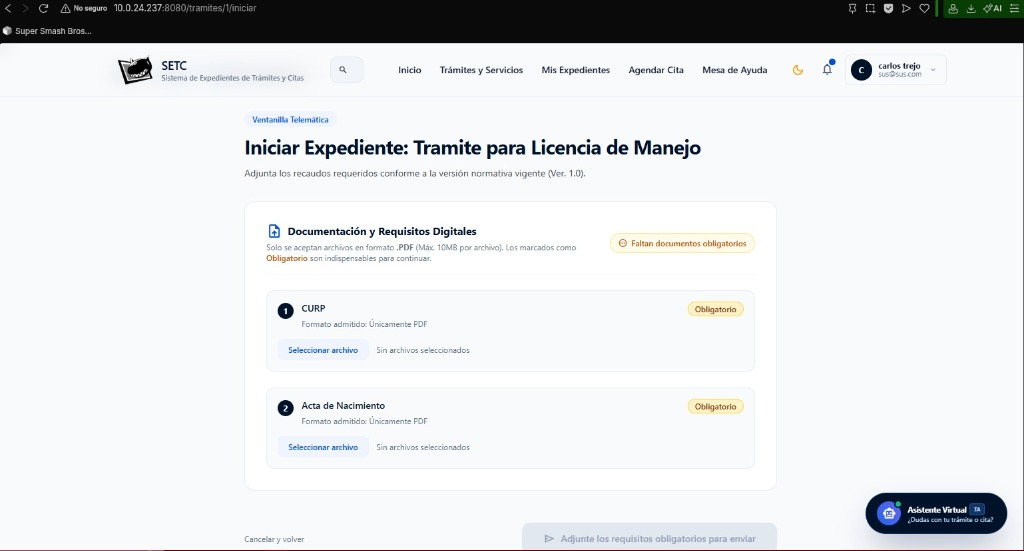
\includegraphics[width=15cm]{imagenes/radicacion_formulario.jpg}
    \caption{Formulario digital de radicación de expediente y carga de recaudos en SETC.}
    \label{fig:radicacion_formulario}
\end{figure}

\subsection{Módulo de Asistente de Inteligencia Artificial (IA)}

Para optimizar la interacción del ciudadano con la plataforma y reducir la tasa de rechazo por errores documentales, se implementó un Asistente de Inteligencia Artificial accesible de forma interactiva en la interfaz ciudadana:

\begin{itemize}
    \item \textbf{Orientación en Lenguaje Natural:} El asistente permite a los ciudadanos resolver inquietudes sobre el trámite en curso, las características requeridas en los documentos y los pasos procedimentales a seguir.
    \item \textbf{Soporte en Subsanaciones:} Cuando un usuario recibe una observación pericial, el asistente le ofrece explicaciones sencillas y sugerencias concretas para corregir adecuadamente el recaudo solicitado.
    \item \textbf{Disponibilidad Continua y No Intrusiva:} Diseñado como un componente flotante e interactivo, asiste al administrado sin interferir con el diligenciamiento regular de los formularios.
\end{itemize}

En la Figura \ref{fig:asistente_ia_widget}, se aprecia la ventana interactiva del Asistente Virtual IA respondiendo consultas sobre los recaudos normativos y guiando al solicitante.

\begin{figure}[H]
    \centering
    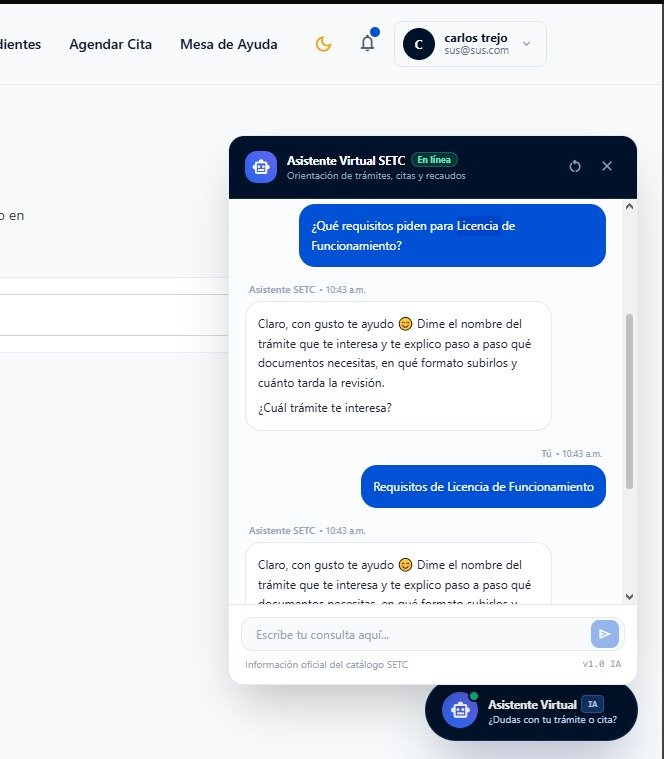
\includegraphics[width=9cm]{imagenes/asistente_ia_widget.jpg}
    \caption{Interfaz conversacional del Asistente de Inteligencia Artificial de SETC.}
    \label{fig:asistente_ia_widget}
\end{figure}

\subsection{Módulo de Trazabilidad y Línea de Tiempo Procedimental Dinámica}

Para solventar la opacidad histórica de las ventanillas tradicionales, se diseñó una línea de tiempo dinámica en vivo sincronizada con el estado transaccional del expediente. Este componente visualiza el progreso en cinco fases institucionales:

\begin{itemize}
    \item \textbf{Fase 1: Radicación:} Confirmación de recepción formal de la solicitud y emisión del folio institucional con sello de tiempo.
    \item \textbf{Fase 2: Asignación Técnica:} Notificación de turno al revisor técnico colegiado, mostrando fecha de recepción y especialista responsable.
    \item \textbf{Fase 3: Evaluación de Recaudos y Subsanaciones:} Estado activo de cotejo documental. Refleja dinámicamente si los documentos se encuentran en análisis, si existen subsanaciones en curso enviadas por el administrado o si el expediente fue calificado favorablemente.
    \item \textbf{Fase 4: Dictamen Técnico de Calificación:} Emisión formal del dictamen pericial aprobatorio o denegatorio derivado del análisis de fondo.
    \item \textbf{Fase 5: Resolución Final:} Firma de la cédula resolutiva institucional, generación del documento resolutivo oficial en PDF y puesta a disposición del ciudadano con código QR de verificación pública.
\end{itemize}

En la Figura \ref{fig:timeline_5fases}, se observa la barra de estado procedural sincronizada en vivo, reflejando el progreso del trámite a través de sus fases institucionales.

\begin{figure}[H]
    \centering
    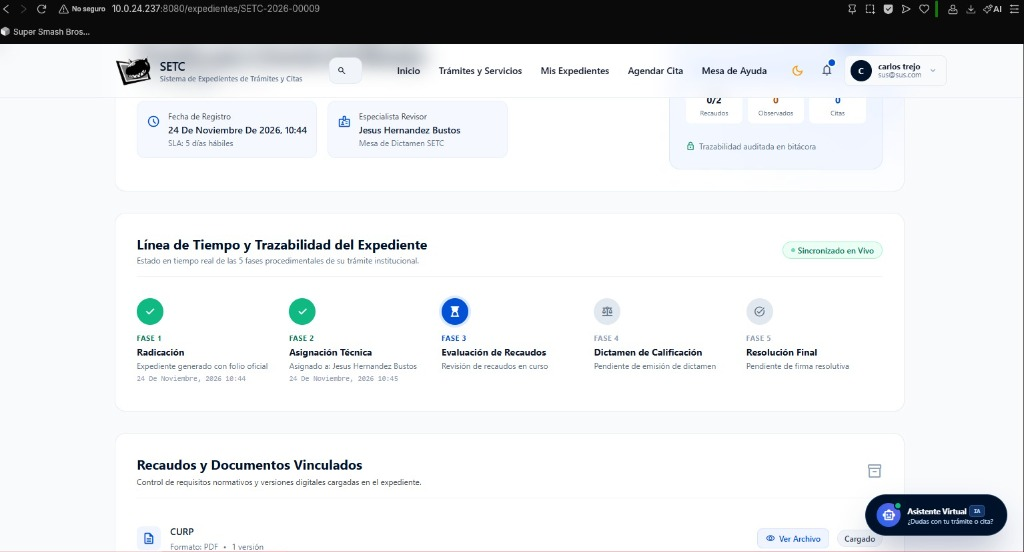
\includegraphics[width=15.5cm]{imagenes/timeline_5fases.jpg}
    \caption{Línea de tiempo procedural dinámica en cinco fases del sistema SETC.}
    \label{fig:timeline_5fases}
\end{figure}

\subsection{Módulo de Mesa de Dictamen y Evaluación Documental}

La Mesa de Dictamen constituye el espacio de trabajo operativo del personal técnico. Proporciona una interfaz ergonómica orientada a la eficiencia pericial:

\begin{itemize}
    \item \textbf{Visor Integrado de Recaudos:} Permite al revisor previsualizar directamente en pantalla los documentos cargados, cotejando requisitos normativos sin necesidad de descargas externas.
    \item \textbf{Calificación Granular por Requisito:} Cada documento es calificado de forma independiente bajo tres estados normativos: \textbf{Aprobado}, \textbf{Observado} o \textbf{Rechazado}.
    \item \textbf{Gestión de Observaciones y Subsanaciones:} Cuando un requisito no satisface el estándar técnico, el revisor redacta una observación puntual. El sistema notifica al ciudadano y habilita en su portal una ventana de subsanación contextual.
    \item \textbf{Control de Flujo Reactivo ante Rechazo:} Si un requisito o el dictamen general es catalogado como \textbf{Rechazado}, el sistema bloquea inmediatamente la recepción de subsanaciones y presenta en el portal ciudadano una alerta explícita en color carmesí indicando la denegación formal del trámite e instruyendo el inicio de una nueva solicitud en caso de requerirlo.
    \item \textbf{Aprobación Consolidada:} Al emitirse un dictamen global \textbf{Aprobado}, los recaudos en estado subsanado o pendiente se promocionan automáticamente al estado final de aprobación, desbloqueando el avance inmediato de la línea de tiempo a la fase resolutiva.
\end{itemize}

En la Figura \ref{fig:mesa_dictamen_revisor}, se muestra la consola de calificación documental del revisor técnico con el visor integrado de expedientes en PDF.

\begin{figure}[H]
    \centering
    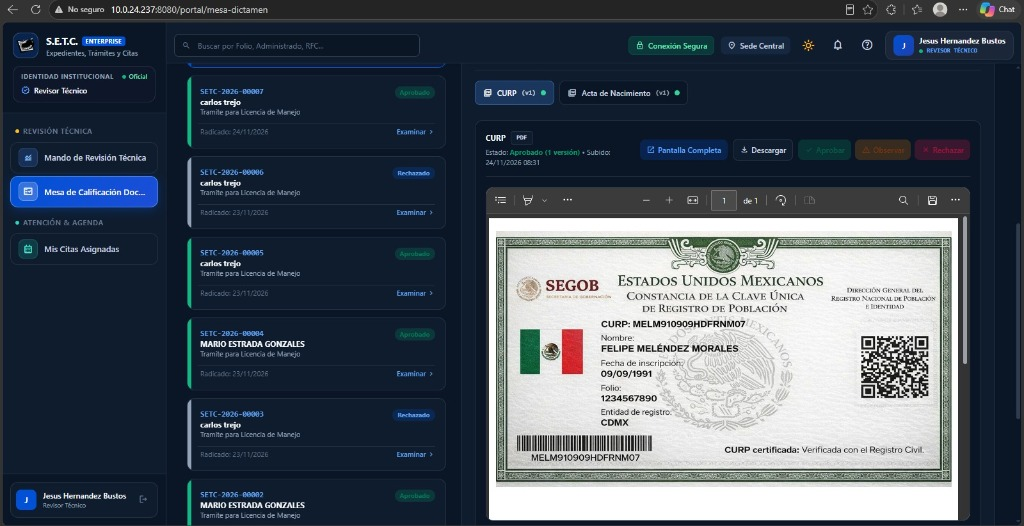
\includegraphics[width=15.5cm]{imagenes/mesa_dictamen_revisor.jpg}
    \caption{Consola de Mesa de Dictamen técnico y visor pericial de recaudos.}
    \label{fig:mesa_dictamen_revisor}
\end{figure}

En la Figura \ref{fig:ventana_subsanaciones}, se presenta la interfaz habilitada al administrado ante observaciones emitidas, permitiéndole enviar respuestas y cargar archivos corregidos.

\begin{figure}[H]
    \centering
    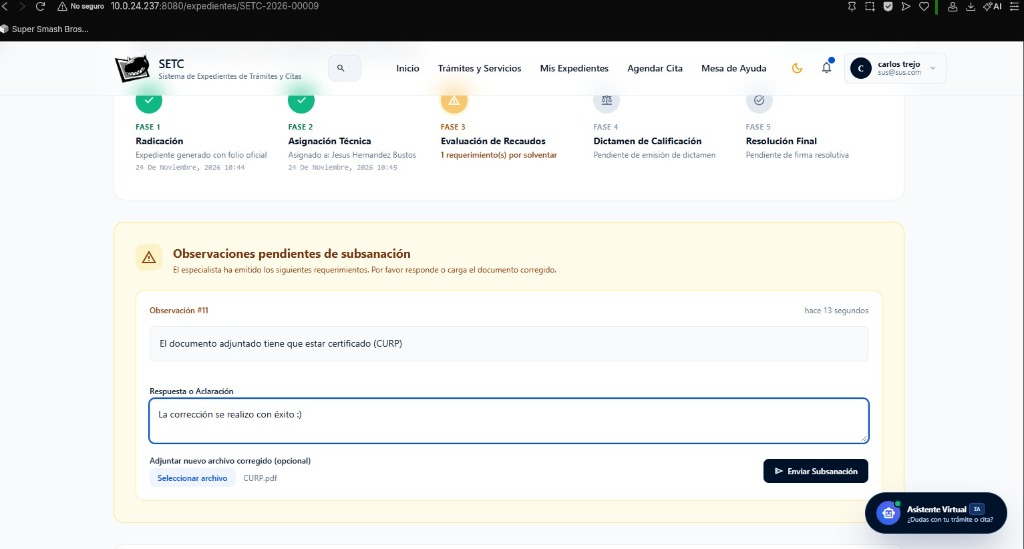
\includegraphics[width=15.5cm]{imagenes/ventana_subsanaciones.jpg}
    \caption{Módulo de atención de observaciones y envío de subsanaciones ciudadanas.}
    \label{fig:ventana_subsanaciones}
\end{figure}

\subsection{Módulo de Supervisión y Asignación de Cargas Operativas}

El módulo de supervisión proporciona una vista consolidada para la administración del personal técnico revisor:

\begin{itemize}
    \item \textbf{Panel de Distribución de Carga:} Permite al supervisor monitorear la cantidad de expedientes turnados a cada revisor técnico, facilitando una asignación equitativa del trabajo institucional.
    \item \textbf{Reasignación y Turnado Pericial:} El supervisor dispone de controles operativos para canalizar expedientes a revisores específicos o reasignar casos según la disponibilidad del personal en turno.
\end{itemize}

En la Figura \ref{fig:panel_supervision}, se detalla la consola del supervisor con las métricas del equipo técnico y la administración de expedientes asignados.

\begin{figure}[H]
    \centering
    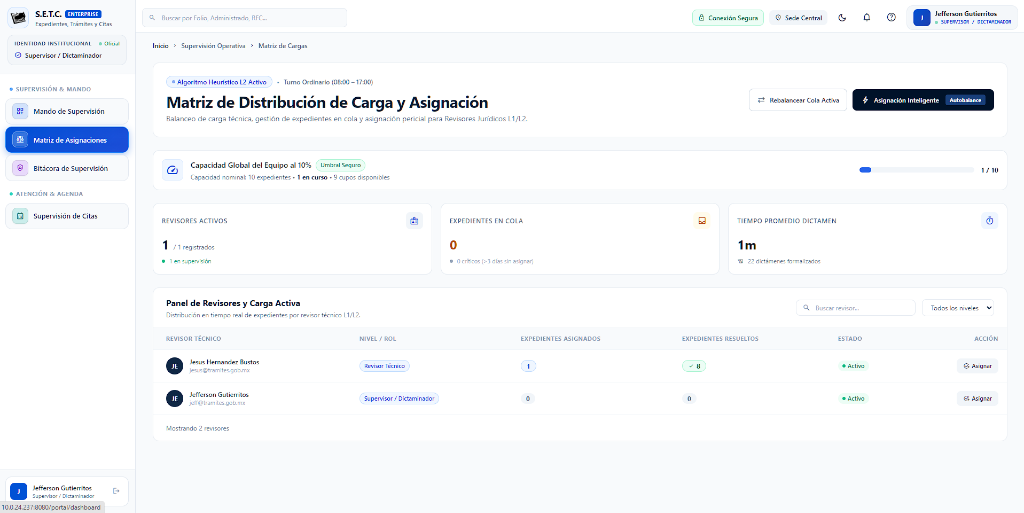
\includegraphics[width=15.5cm]{imagenes/panel_supervision.png}
    \caption{Matriz de distribución de cargas y supervisión operativa de revisores.}
    \label{fig:panel_supervision}
\end{figure}

\subsection{Módulo de Agendamiento de Citas y Pases Digitales con Código QR}

Para trámites que requieran presencia física o cotejo de documentos originales, el sistema integra una solución telemática de citas:

\begin{itemize}
    \item \textbf{Selección de Sede y Calendario:} El ciudadano visualiza la disponibilidad en tiempo real por módulo y fecha, evitando duplicidades de horarios mediante bloqueos transaccionales.
    \item \textbf{Pase Digital de Cita:} Confirmada la reserva, se expide un pase digital descargable e imprimible que incorpora los datos del titular, trámite, sede, horario y un \textbf{Código QR} criptográficamente firmado.
    \item \textbf{Validación Telemática de Asistencia:} El personal de control de acceso en ventanilla escanea el código QR con cualquier dispositivo móvil para validar instantáneamente la autenticidad del turno en la base de datos central y registrar el ingreso del solicitante.
\end{itemize}

En la Figura \ref{fig:pase_cita_qr}, se muestra el pase digital oficial emitido al ciudadano, incorporando el código QR para su validación presencial en ventanilla.

\begin{figure}[H]
    \centering
    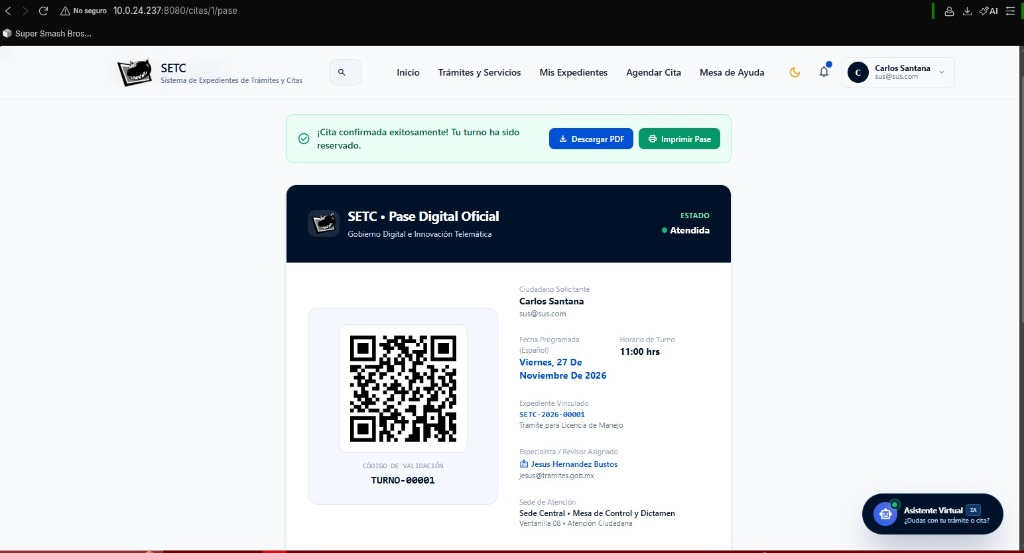
\includegraphics[width=12cm]{imagenes/pase_cita_qr.jpg}
    \caption{Pase digital oficial de cita con código QR de verificación telemática.}
    \label{fig:pase_cita_qr}
\end{figure}

\subsection{Módulo de Auditoría y Bitácora Transaccional Forense}

En cumplimiento de las normativas de transparencia y rendición de cuentas, la plataforma incorpora un subsistema de auditoría inmutable:

\begin{itemize}
    \item Cada cambio de estado de solicitud, dictamen emitido, archivo reemplazado o reasignación de revisor queda consignado en la tabla \texttt{bitacoras}.
    \item Se registra la identidad del usuario ejecutor, dirección IP de origen, huella digital del navegador (\textit{User-Agent}), marca de tiempo exacta con precisión de milisegundos y el estado de los datos antes y después de la operación (\textit{JSON payloads}).
\end{itemize}

En la Figura \ref{fig:bitacora_auditoria}, se ilustra el panel de auditoría institucional donde se registran de forma inmutable todas las transacciones realizadas sobre los expedientes.

\begin{figure}[H]
    \centering
    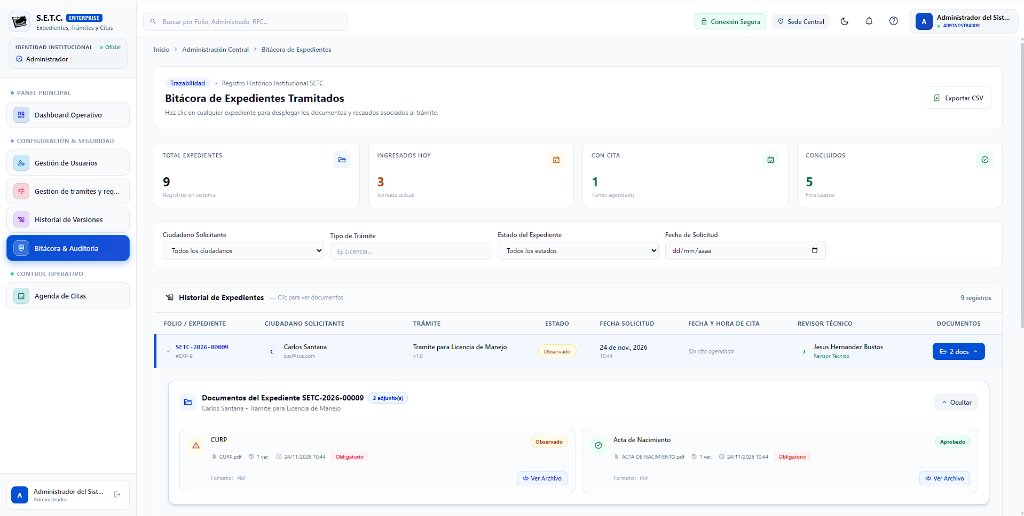
\includegraphics[width=15.5cm]{imagenes/bitacora_auditoria.jpg}
    \caption{Bitácora de auditoría transaccional e historial institucional de expedientes.}
    \label{fig:bitacora_auditoria}
\end{figure}

\section{Aseguramiento de Calidad y Pruebas del Sistema}

Para certificar la confiabilidad, estabilidad y seguridad del sistema ante fallos o accesos no autorizados, se adoptó una estrategia de aseguramiento continuo de la calidad respaldada por el framework de pruebas \textbf{Pest PHP v3}.

\subsection{Diseño y Ejecución de la Suite de Pruebas}

Se implementaron pruebas de integración y de características (\textit{Feature Tests}) que simulan de extremo a extremo las interacciones de los cuatro roles de usuario. Entre los escenarios críticos cubiertos se destacan:

\begin{itemize}
    \item \textbf{Autenticación y Redirección por Rol:} Verificación del redireccionamiento contextual de usuarios tras iniciar sesión hacia sus paneles correspondientes (Portal Ciudadano, Mesa de Dictamen o Consola Administrativa).
    \item \textbf{Restricción de Acceso a Expedientes Ajenos:} Pruebas de seguridad negativa confirmando que un usuario ciudadano recibe un código HTTP 403 al intentar acceder a solicitudes de terceros o a rutas operativas del personal técnico.
    \item \textbf{Carga y Validación de Archivos:} Pruebas de inyección de archivos no permitidos (ejecutables, imágenes, archivos vacíos) confirmando el rechazo estricto y la aceptación exclusiva de documentos PDF válidos menores a 10 MB.
    \item \textbf{Ciclo de Subsanación y Avance de Línea de Tiempo:} Validación del flujo completo donde un revisor emite una observación, el ciudadano adjunta una subsanación, el revisor aprueba el recaudo y la línea de tiempo se actualiza de manera coherente sin inconsistencias de estado.
    \item \textbf{Asignación de Cargas y Matriz de Revisores:} Pruebas de la asignación formal de expedientes comprobando la correcta distribución y visibilidad en el panel del revisor asignado.
\end{itemize}

La totalidad de las pruebas automatizadas (72 casos de prueba con más de 260 aserciones) se ejecutan con éxito en el pipeline de validación continua con un tiempo de respuesta inferior a 4 segundos.

\subsection{Infraestructura de Despliegue con Docker}

El entorno operativo del sistema se empaqueta mediante contenedores \textbf{Docker} con configuración multi-etapa (\textit{multi-stage builds}), garantizando homogeneidad entre los entornos de desarrollo, pruebas y producción:

\begin{itemize}
    \item \textbf{Contenedor de Aplicación (PHP-FPM):} Basado en imágenes optimizadas de PHP 8.4 Alpine, con extensiones requeridas para el motor de bases de datos, procesamiento de cadenas criptográficas y manipulación de documentos PDF.
    \item \textbf{Servidor Web (Nginx / Vite):} Servidor de alto rendimiento configurado para servir activos estáticos optimizados mediante compresión Gzip/Brotli y canalizar peticiones dinámicas a través de sockets FastCGI.
    \item \textbf{Aislamiento y Volúmenes de Almacenamiento:} Los documentos de los expedientes y los registros de auditoría se almacenan en volúmenes persistentes desacoplados del ciclo de vida del contenedor, garantizando la integridad y permanencia de la información institucional.
\end{itemize}
